%%%%%%%%%%%%%%%%%%%%%%%%%%%%%%%%%%%%%%%%%%%%%%%%%%%%%%%%%%%%%%%%%%%%%%
% Problem statement
\begin{statement}[
  problempoints=110,
  timelimit=1 second,
  memorylimit=512 MiB,
]{Zvijezda}

Mirko and Slavko are spending their free time playing with polygons and watching
a new season of \textit{The Biggest Loser}. Mirko recently drew a convex polygon
with an even number of vertices $N$. Slavko then considered each pair of oposite
sides (two sides are opposite if there are $\frac{N}{2}-1$ sides between them),
drew straight lines that lie on those sides and colored them along with the
part of the plane that lies between them and contains the polygon. Finally,
Mirko found a set of $Q$ points and decided to challenge Slavko to answer for
each point whether it lies in the colored or uncolored part of the plane.

The new episode of \textit{The Biggest Loser} is about to start and Slavko
doesn't have the time to answer Mirko's queries. Can you help him?

%%%%%%%%%%%%%%%%%%%%%%%%%%%%%%%%%%%%%%%%%%%%%%%%%%%%%%%%%%%%%%%%%%%%%%
% Input
\subsection*{Input}
The first line contains an integer $T$ which is used as a parameter for
generating Mirko's queries. This number can be either $0$ or $1$.

The second line contains an even integer $N$ from the task description.

Each of the next $N$ lines contains two integers $X_i$, $Y_i$
$(0 \le |Xi|, |Yi| \le 10^9)$ which represent one of the polygon's vertices. You
can assume that the vertices are given in the counter clockwise order and that
no three successive vertices are collinear.

The next line contains an integer $Q$ from the task description.

Each of the next $Q$ lines contains two integers $A_i$, $B_i$
$(0 \le |Ai|, |Bi| \le 2\cdot10^{18})$ which are used as parameters for
generating the point in the $i$-th of Mirko's queries.

Let $X_i$ be equal to the number of points in the first $i$ (inclusive) of
Mirko's queries that lie in the colored part of the plane. Naturally, $X_0=0$.
The point of Mirko's $i$-th query should then be generated as:

\[P_i = (A_i \oplus (T \cdot X_{i-1}^{3}), B_i \oplus (T \cdot X_{i-1}^{3}))\]
where $\oplus$ represents the bitwise xor operation.

%%%%%%%%%%%%%%%%%%%%%%%%%%%%%%%%%%%%%%%%%%%%%%%%%%%%%%%%%%%%%%%%%%%%%%
% Output
\subsection*{Output}
The $i$-th line of output should contain the word \texttt{"DA"} (YES in
Croatian) if the point from $i$-th of Mirko's queries lies in the colored
part of the plane. Otherwise, the $i$-th line should contain the word
\texttt{"NE"} (NO in Croatian).

%%%%%%%%%%%%%%%%%%%%%%%%%%%%%%%%%%%%%%%%%%%%%%%%%%%%%%%%%%%%%%%%%%%%%%
% Scoring
\subsection*{Scoring}
{\renewcommand{\arraystretch}{1.4}
  \setlength{\tabcolsep}{6pt}
  \begin{tabular}{ccl}
 Subtask & Score & Constraints \\ \midrule
  1 & 20 & $1 \le N, Q \le 2000$, $T = 0$ \\
  2 & 30 & $1 \le N, Q \le 10^5$, $T = 0$ \\
  3 & 60 & $1 \le N, Q \le 10^5$, $T = 1$
\end{tabular}}

%%%%%%%%%%%%%%%%%%%%%%%%%%%%%%%%%%%%%%%%%%%%%%%%%%%%%%%%%%%%%%%%%%%%%%
% Examples
\subsection*{Examples}
\begin{tabularx}{\textwidth}{X'X'X}
\sampleinputs{test/zvijezda.dummy.in.1}{test/zvijezda.dummy.out.1} &
\sampleinputs{test/zvijezda.dummy.in.2}{test/zvijezda.dummy.out.2} &
\sampleinputs{test/zvijezda.dummy.in.3}{test/zvijezda.dummy.out.3}
\end{tabularx}

\textbf{Clarification of the second example:}
\begin{figure}[H]
\centering
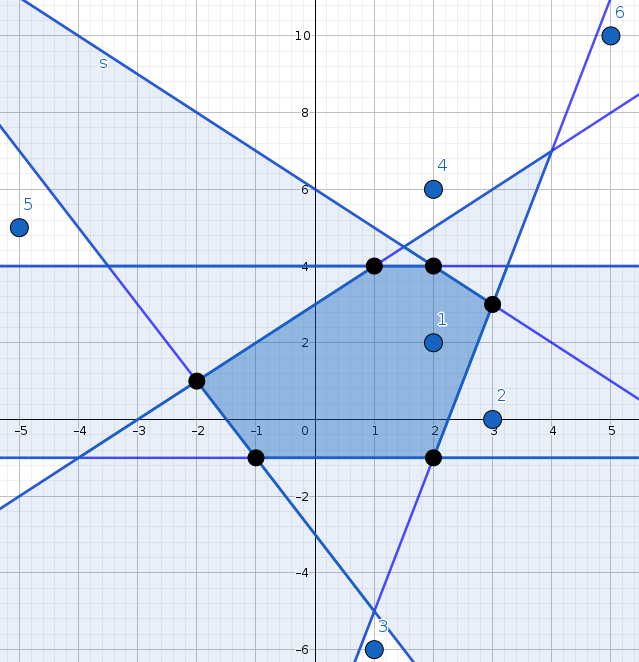
\includegraphics[width=0.5\textwidth]{img/zvijezda_clar.png}
\end{figure}

\textbf{Clarification of the third example:}
The colored parts of the plane are the same as in the second example and
the points in Mirko's queries are:
$(2, 2)$, $(2, 1)$, $(9, -14)$, $(25, 29)$,
$(-32, 30)$ and $(30, 17)$.

%%%%%%%%%%%%%%%%%%%%%%%%%%%%%%%%%%%%%%%%%%%%%%%%%%%%%%%%%%%%%%%%%%%%%%
% We're done
\end{statement}

%%% Local Variables:
%%% mode: latex
%%% mode: flyspell
%%% ispell-local-dictionary: "croatian"
%%% TeX-master: "../hio.tex"
%%% End:
